%%%%%%%%%%%%%%%%%%%%%%%%%%%%%%%%%%%%%%%%%
% Beamer Presentation
% LaTeX Template
% Version 1.0 (10/11/12)
%
% This template has been downloaded from:
% http://www.LaTeXTemplates.com
%
% License:
% CC BY-NC-SA 3.0 (http://creativecommons.org/licenses/by-nc-sa/3.0/)
%
%%%%%%%%%%%%%%%%%%%%%%%%%%%%%%%%%%%%%%%%%

%----------------------------------------------------------------------------------------
%	PACKAGES AND THEMES
%----------------------------------------------------------------------------------------

\documentclass{beamer}

\mode<presentation> {

% The Beamer class comes with a number of default slide themes
% which change the colors and layouts of slides. Below this is a list
% of all the themes, uncomment each in turn to see what they look like.

%\usetheme{default}
%\usetheme{AnnArbor}
%\usetheme{Antibes}
%\usetheme{Bergen}
%\usetheme{Berkeley}
\usetheme{Berlin}
%\usetheme{Boadilla}
%\usetheme{CambridgeUS}
%\usetheme{Copenhagen}
%\usetheme{Darmstadt}
%\usetheme{Dresden}
%\usetheme{Frankfurt}
%\usetheme{Goettingen}
%\usetheme{Hannover}
%\usetheme{Ilmenau}
%\usetheme{JuanLesPins}
%\usetheme{Luebeck}
%\usetheme{Madrid}
%\usetheme{Malmoe}
%\usetheme{Marburg}
%\usetheme{Montpellier}
%\usetheme{PaloAlto}
%\usetheme{Pittsburgh}
%\usetheme{Rochester}
%\usetheme{Singapore}
%\usetheme{Szeged}
%\usetheme{Warsaw}

% As well as themes, the Beamer class has a number of color themes
% for any slide theme. Uncomment each of these in turn to see how it
% changes the colors of your current slide theme.

%\usecolortheme{albatross}
%\usecolortheme{beaver}
%\usecolortheme{beetle}
%\usecolortheme{crane}
%\usecolortheme{dolphin}
%\usecolortheme{dove}
%\usecolortheme{fly}
%\usecolortheme{lily}
%\usecolortheme{orchid}
%\usecolortheme{rose}
%\usecolortheme{seagull}
%\usecolortheme{seahorse}
%\usecolortheme{whale}
%\usecolortheme{wolverine}

%\setbeamertemplate{footline} % To remove the footer line in all slides uncomment this line
%\setbeamertemplate{footline}[page number] % To replace the footer line in all slides with a simple slide count uncomment this line

%\setbeamertemplate{navigation symbols}{} % To remove the navigation symbols from the bottom of all slides uncomment this line
}

\usepackage{graphicx} % Allows including images
\usepackage{booktabs} % Allows the use of \toprule, \midrule and \bottomrule in tables
%\usepackage[brazilian]{babel}
\usepackage[utf8]{inputenc}
\usepackage{listings}
\usepackage{amsmath}
\usepackage{amsfonts}
\usepackage{pdfpages}
\usepackage{textpos}

\graphicspath{ {img/} }

%----------------------------------------------------------------------------------------
%	TITLE PAGE
%----------------------------------------------------------------------------------------

\title[Generating Acrostics via Paraphrasing and Heuristic Search]{Generating Acrostics via Paraphrasing and Heuristic Search $-$ Final Presentation} % The short title appears at the bottom of every slide, the full title is only on the title page

\author[Bruno, Fernando, Jürgen, William]{Bruno Soares Fillmann\\
Fernando Bombardelli da Silva\\
Jürgen Bauer\\
William Bombardelli da Silva
} % Your name
\institute[TU Berlin] % Your institution as it will appear on the bottom of every slide, may be shorthand to save space
{
Technische Universität Berlin \\ % Your institution for the title page
Datenbanksysteme und Informationsmanagement \\
DBPRO – Database Projects (WS 2014/2015) \\
\medskip
%\textit{fbdasilva@inf.ufrgs.br} % Your email address
}
\date{09.02.2015} % Date, can be changed to a custom date

\begin{document}

\begin{frame}
\titlepage % Print the title page as the first slide
\end{frame}

\begin{frame}
\frametitle{Organization} % Table of contents slide, comment this block out to remove it
\tableofcontents % Throughout your presentation, if you choose to use \section{} and \subsection{} commands, these will automatically be printed on this slide as an overview of your presentation
\end{frame}

%----------------------------------------------------------------------------------------
%	PRESENTATION SLIDES
%----------------------------------------------------------------------------------------

%------------------------------------------------
\section{Goals} % Sections can be created in order to organize your presentation into discrete blocks, all sections and subsections are automatically printed in the table of contents as an overview of the talk
%------------------------------------------------

\begin{frame}
\frametitle{The Problem}
\begin{itemize}
\item Given a text T and an acrostic X, find a paraphrased version of T that encodes X in the first letters of each line.
\end{itemize}
Original Text: \footnote{\tiny \url{http://www.gutenberg.org/browse/languages/de}} \\
\texttt{\tiny Zuerst wollte er mit dem unteren Teil seines Körpers aus dem Bett \\
hinauskommen, aber dieser untere Teil, den er übrigens noch nicht \\
gesehen hatte und von dem er sich auch keine rechte Vorstellung machen \\
konnte, erwies sich als zu schwer beweglich; es ging so langsam; und \\
als er schließlich, fast wild geworden, mit gesammelter Kraft, ohne \\
Rücksicht sich vorwärtsstieß, hatte er die Richtung falsch gewählt...\\}

Result Text: \\

\texttt{\scriptsize{Z}\tiny uerst wollte er mit dem unteren Teil seines Körpers a-\\
\scriptsize{u}\tiny s dem Bett hinauskommen, aber dieser untere Teil, den\\
\scriptsize{e}\tiny r übrigens noch nicht gesehen hatte und von dem er sich auch keine\\
\scriptsize{r}\tiny echte Vorstellung machen konnte, erwies sich als zu\\
\scriptsize{s}\tiny chwer beweglich; es ging so langsam; und als er schließlich, fas-\\
\scriptsize{t}\tiny \ wild geworden, mit gesammelter Kraft, ohne Rücksicht sich\\
vorwärtsstieß, hatte er die Richtung falsch gewählt...\\}
\end{frame}

\begin{frame}
\frametitle{Goal of the Project}
%\begin{itemize}	%\item
\textbf{Goal:} Implement the methods and techniques to generate acrostics for the German language as described in the paper \emph{Generating Acrostics via Paraphrasing and Heuristic Search} of Benno Stein, Matthias Hagen, and Christof Bräutigam, published in August 2014 \cite{Stein}. \par

\textbf{Main idea of the algorithm:}
	\begin{itemize}
	\item Modeled as a search problem in a tree.
	\item The vertices are states (texts) and the edges are operations over states.
	\item Artificial intelligence is applied for the search strategy (A* Algorithm).
	\end{itemize}
	
	%\item Use the A* algorithm to solve the search problem.
	%\item Apply the heuristic with proper modifications for the German language.
	%\item Find datasources in German (Thesaurus, hyphenation rules, etc.).
	%\item Implement the operators described in the paper to achieve results in German texts.
%\end{itemize}
\end{frame}

\begin{frame}
\begin{figure}[H]
\vspace*{-15pt}
\hspace*{-25pt}
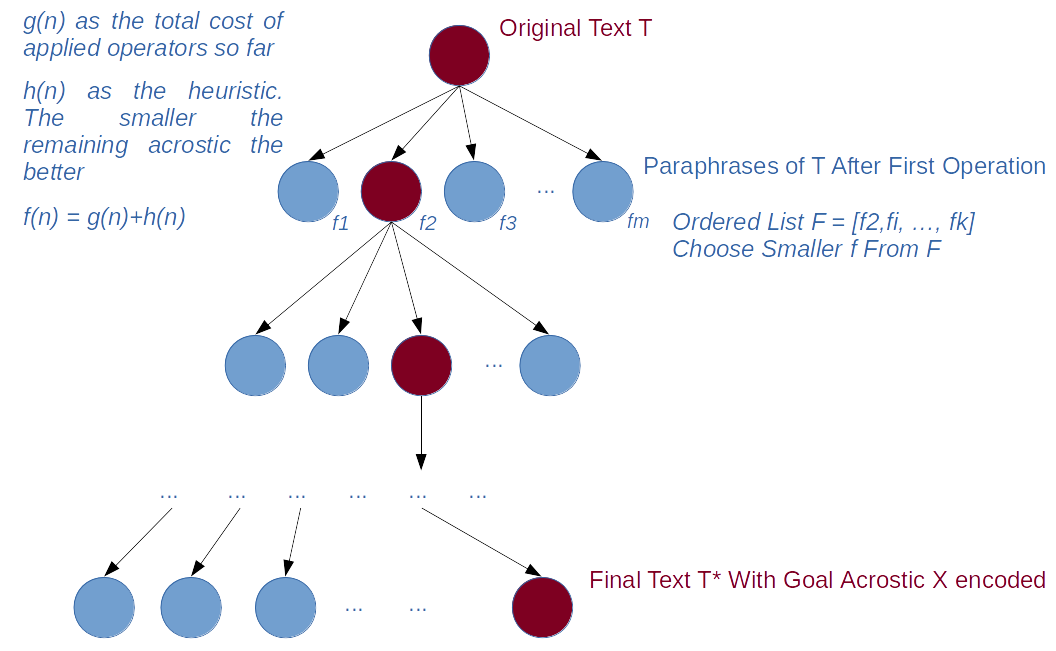
\includegraphics[scale=0.44]{a_star.png}
\end{figure}
\end{frame}

%\begin{frame}
%\frametitle{Goal of the Project}
%\begin{itemize}
%	\item Set proper costs for each of the operators.
%	\item Collect texts to use as examples.
%	\item Solve the problems in a reasonable time.
%	\item Evaluate the efficiency of our algorithm.
%	\item Evaluate the usage rate of the operators.
%\end{itemize}
%\end{frame}

%-----------------------------------------------
\section{Subtasks}
%------------------------------------------------
\begin{frame}
\frametitle{Subtasks of the original goal}
\begin{itemize}
	\item Understand the paper and the method
	\item Design an architecture for the application	
	\item Collect comparable German text corpora, statistics and libraries
	(TEX Hyphenation, NetSpeakAPI, Thesaurus, etc.)
	\item Implement the most promising paraphrasing operators\\
	(line break, hyphenation, wrong 
	hyphenation, word insertion/deletion, synonym, spelling)
	\item Implement the $A^*$-algorithm
	\item Evaluate the results
	
	
	%\item Analyze the problem.
	
	%\item Choose proper technological tools.
\end{itemize}
\end{frame}



%\begin{frame}
%\frametitle{Subtasks from the Original Goals}
%\begin{itemize}
%	\item Choose the most promising operators.
%	\item Implement the best first (A*) algorithm itself.
%	\item Set up a test suite for evaluation of the application.
%	\item Interpret the results from the tests.
%\end{itemize}
%\end{frame}

%------------------------------------------------
\section{Method}
%------------------------------------------------
\begin{frame}
\frametitle{How have we reached the goals?}
\begin{itemize}
	\item UML-diagram for the application
	\item Sequence diagram for the $A^*$-algorithm
	\item Developed the application in Java 8 with Netbeans
	\item Used various libraries, web services and databases to implement
	the operators
	\item Implemented a test application for evaluating the results, with
	a timeout after 15 min

	
	
	%\item Use NetSpeakAPI for context dependent operators.
	%\item Use the key-value store server (Redis) for the synonyms database.
	%\item Use Open Thesaurus as the German synonyms database.
	%\item Use several Java libraries for hyphenation, line break, etc.
\end{itemize}
\end{frame}


%------------------------------------------------
\section{Difficulties}
%------------------------------------------------
\begin{frame}
\frametitle{Which difficulties did occur?}
\begin{itemize}
	\item Synonym operation only inserts synonyms without considering
	the context (Google N-Gram)
	\item Lack of powerful grammatical operator
	\item NetSpeakAPI doesn't yield many results for the German language
	\item NetSpeakAPI's requests to the web server takes much time
	\item The empirical choice of costs is not optimal for the search
\end{itemize}
\end{frame}



\begin{frame}
\frametitle{Which difficulties did occur?}
\begin{itemize}
	\item Organization of the input text as line:
	\begin{itemize}
		
%		\item no clear separation of operator applications
%		(e.g. various hyphens produced by ensure constraints)
		
		\item More than one letter of the acrostic can be generated at a time, not following the theoretical framework of the $A^*$-algorithm as described in the paper.
		
		\item \textbf{Recommendation:} view the text as one single line and apply
			line break only to generate a letter. When the acrostic is generated,
			break the lines according to the constraints.
	\end{itemize}
\end{itemize}
\end{frame}


%------------------------------------------------
\section{Unreached Goals}
%------------------------------------------------
\begin{frame}
\frametitle{Unreached Goals}
\begin{itemize}
	\item Only the most promising operators were implemented.
	\item No effective operator to generate the first letter of the acrostic.
	\item No operator \textbf{not} mentioned in the paper was coded.
	\item No local databases for \emph{n-gram} were implemented.
	\item No sophisticated quality measures were implemented.
\end{itemize}
\end{frame}



%------------------------------------------------
\section{Example}
%------------------------------------------------
\begin{frame}

\frametitle{Example}
Original Text: \footnote{\tiny \url{http://german.airportljubljana.co/Billig\_nach\_Klagenfurt.php}} \\
\texttt{\scriptsize Billig nach Hamburg. 24/7 taxidienst bietet ihnen kostengünstige und \\
zuverlässige verkehr aus Kiel. Mit erfahrung in der branche wir \\
garantieren die niedrigsten preis nach Hamburg. Gleiche preis gilt \\
auch wenn sie taxi aus Kiel stadt nach Hamburg nehmen. \\}

Final Text: \par

\texttt{\footnotesize{B}\scriptsize illig nach Hamburg. 24/7 taxidienst bietet ihnen kostengünstige \\
\footnotesize{u}\scriptsize nd zuverlässige verkehr aus Kiel. Mit erfahrung in der bran- \\
\footnotesize{c}\scriptsize he wir garantieren ihnen die niedrigsten preis nach \\
\footnotesize{H}\scriptsize amburg. Gleiche preis gilt auch wenn sie taxi aus Kiel stadt nach \\
Hamburg nehmen. \\}
\end{frame}

\begin{frame}
\frametitle{Example}
Original Text: \footnote{\tiny \url{http://www.gutenberg.org/browse/languages/de}} \\
\texttt{\scriptsize Diese war unterdessen in das Aussehen gerückt, was die Gegenwart\\
damals hatte, sie war sehr schön, aber immer traurig, weil sie sich\\
vor ihrem Bräutigam fürchtete und weil sie von den Schwestern, die\\
keinen Mann bekommen, beständig seinetwegen geneckt wurde. Eines Tages\\
rief ein heller Trompetenschall alle drei Schwestern ans...\\
}

Final Text: \par

\texttt{\footnotesize{D}\scriptsize iese war unterdessen in das Aussehen gerückt, was die Gegenwart\\
\footnotesize{i}\scriptsize n jenen tagen hatte, sie war sehr schön, aber immer traurig, weil si-\\
\footnotesize{e}\scriptsize \ sich vor ihrem Bräutigam fürchtete und weil sie von den Schwe-\\
\footnotesize{s}\scriptsize tern, die keinen Mann bekommen, beständig seinetwegen geneckt wurde.\\
\footnotesize{E}\scriptsize ines Tages rief ein heller Trompetenschall alle drei Schwestern ans...\\}
\end{frame}

%------------------------------------------------

%------------------------------------------------
\section{Results}
%------------------------------------------------
\begin{frame}
\frametitle{Results $-$ Evaluation}
\begin{itemize}
	\item 100 Texts.
	\item 4 different ways.
		\begin{description}
			\item[A* + Self-referential:] Regular A* as the algorithm and the first word of the text as the acrostic.
			\item[A* + Most Common:] Regular A* as the algorithm and the most common word in German, that starts with the first letter of the text, as the acrostic.
			\item[Greedy A* + Self-referential:] Greedy A* (ignore costs of operations) as the algorithm and the first word of the text as the acrostic.
			\item[Greedy A* + Most Common:] Greedy A* as the algorithm and the most common word in German, that starts with the first letter of the text, as the acrostic.
		\end{description}
\end{itemize}
\end{frame}

\begin{frame}
\frametitle{Results}
% show the tables of evaluation (from our paper), comment it (1 Slide)

\begin{small}
\begin{table}[h]
\centering
\begin{tabular}{p{2.4cm} | p{1.3cm} | p{1.3cm} | p{1.3cm} | p{1.3cm} | p{1.3cm}}
	\hline
	\textbf{Configuration} & \textbf{Success Rate} & \textbf{Success Runtime} & \textbf{Nodes When Success} & \textbf{Timeout Rate} & \textbf{Nodes When Timeout} \\ \hline
	\textbf{A* + Self-referential}	& 37,62\%	& 31,97 s	& 46112,82	& 62,38\%	& 675794,78 \\ \hline
	\textbf{A* + Most Common}		& 64,36\%	& 29,74 s	& 52547,68	& 35,64\%	& 568845,14 \\ \hline
	\textbf{Greedy A* + Self-referential}	& 60,40\%	& 30,64 s	& 24033,31	& 39,60\%	& 488660,52 \\ \hline
	\textbf{Greedy A* + Most Common}	& 76,24\%	& 9,40 s	& 24639,19	& 23,76\%	& 304303,41 \\ \hline
\end{tabular}
\label{tab:results}
\caption{Experimental results}
\end{table}
\end{small}

\end{frame}

\begin{frame}
\frametitle{Results $-$ Frequency of the operators}
% show the tables of evaluation (from our paper), comment it (1 Slide)

\begin{small}
\begin{table}[h]
\centering
\begin{tabular}{l | l | l}
	\hline
	\textbf{Operation} &	\textbf{A*} &	\textbf{Greedy A*} \\ \hline
	\textbf{LineBreak} &	23,74\% &	14,29\% \\
	\textbf{WrongHyphenation} &	39,39\% &	31,63\% \\
	\textbf{Hyphenation} &	5,05\% &	0,34\% \\
	\textbf{WordInsertionDeletion} &	0,51\% &	0,34\% \\
	\textbf{Synonym} &	29,80\% &	45,58\% \\
	\textbf{WrongSpelling} &	1,52\% &	7,82\% \\
	\hline
\end{tabular}
\label{tab:operations_freq}
\caption{Operations employment frequency}
\end{table}
\end{small}

\end{frame}
%------------------------------------------------

%------------------------------------------------
% Bibliography
%------------------------------------------------
\section{References}
%------------------------------------------------

\begin{frame}
\frametitle{References}
\scriptsize
\begin{thebibliography}{1}
\bibitem{Stein}
	Benno Stein, Matthias Hagen, and Christof Bräutigam. \emph{Generating Acrostics via Paraphrasing and Heuristic Search}. \\
	In Junichi Tsujii and Jan Hajic, editors, 25th International Conference on Computational Linguistics (COLING 14), pages 2018-2029, August 2014. Association for Computational Linguistics.
\bibitem{Netspeak}
	Martin Potthast, Martin Trenkmann, and Benno Stein.
	\emph{Netspeak: Assisting Writers in Choosing Words}. \\
	In Cathal Gurrin et al, editors, Advances in Information Retrieval. 32nd European Conference on Information Retrieval (ECIR 10) volume 5993 of Lecture Notes in Computer Science, pages 672, Berlin Heidelberg New York, March 2010. Springer.
\bibitem{FirstLetterFrequencies}
\emph{Private Communication} with Rainer Perkuhn,
Institut für Deutsche Sprache Programmbereich Korpuslinguistik, via Email, in Dezember 2014. He send us two files of an old study of Cyril Belica, including the first letter frequencies.
\bibitem{AStar}
	Dechter, Rina; Pearl, Judea. \emph{Generalized best-first search strategies and the optimality of A*}. Journal of the ACM (JACM), Volume 32 Issue 3, Pages 505-536, New York, July 1985.
\end{thebibliography}
\end{frame}
%------------------------------------------------

\begin{frame}
\Huge{\centerline{Questions?}}
\end{frame}

%----------------------------------------------------------------------------------------

\end{document}
